\chapter{Skill Design} %\inote{ (was: Implementation) Dienstabfrage}}
\label{mainone}
%DELETEME: In this chapter you start addressing your actual problem. Therefore, it makes often sense to make a detailed problem analysis first (if not done in introduction). You should be sure about what to do and how. As writtin in the background part, it might also make sense to include complex background information or papers you are basing on in this analysis. If you are solving a software problem, you should follow the state of the art of software development which basically includes: problem analysis, design, implementation, testing, and deployment. Maintenance is often also described but I believe this will not be required for most theses. Code should be placed in the appendix unless it is solving an essential aspect of your work.



\todo{\textit{moved from availability section in choice of platform:}\\
We choose to offer our skill only in Germany because our Skill's functionality is specific only within this geographical region. For that we configure the Skill to handle English (US) and German.\\
Consequently we will two interaction models and two handlers. \\
say why we do it like this 3ashan each language group has a different interest although we can do a handler function for two languages but we prefer not to 3ashan ne3melha schöne und nicht systematische implementierung.
}











\begin{table}[h]
	\caption[Interaction Model Schema]{\href{https://developer.amazon.com/docs/smapi/interaction-model-schema.html}{Interaction Model Schema (Skill Management API)~\cite{alexaDesignGuide} }}\label{interactionModel}
	\begin{tabularx}{\textwidth}{|l | l l l | }
		Field	&	Type	&	Description		&	Required \\ \hline
		\lstinline|languageModel| &	object	& Conversational primitives for the skill	& yes\\
		\_\_\lstinline|invocationName| &	object	& Invocation name of the skill	& yes\\
		\_\_\lstinline|intents| &	array	& Intents and their slots	& yes\\
		\_\_\_\_\lstinline|slots| (Intent Slots) & array & List of slots within the intent	& no\\
		\_\_\lstinline|types| &	array	& Custom slot types		& no\\
		\_\_\lstinline|samples|	& array	 & Sample utterances for the intent	& no\\
		
		dialog & & & \\
		elicitationRequired & & & \\
		elicitation & & & \\
		type (slot type) & & & \\
		name (slot name) & & & \\
		
		prompts & & & \\
		\_\_ id  & & & \\
		\_\_\_\_variations  & & & \\
		\_\_\_\_\_\_type  & & & \\
		\_\_\_\_\_\_value  & & & \\ \hline
		
	\end{tabularx}			
\end{table}






























\todo{
	intro on structure of chapter\\
- to then elaborate on implementation requirements in section \ref{frameworks_structs}. 
- on Skill design: \href{https://medium.com/the-mission/nobody-cares-about-your-amazon-alexa-skill-ac14bd080327}{nobody cares abt ur skill}
- functional requirements (although this is not OCL now, but requiring an SSL cert.) / non-functional (bot muss höflich sein)
}

we say first decision was to go for alexa so we see what we kind of frameworks we need around it

\todo{
	then talk about how you researched on alexa's available skills and found out that the e-Government sector is underrepresented and hence you chose this as ur analyzed scenario.\\
	%%% move to section \ref{choiceOfPlatform}
	fluidly contiuning from intro and background:\\
	- since among Apple and Google it hast the voice-first devices best equipped for its platform, a user base larger then its competition and provides the most mature API and SDKs.\\
	
	- We choose this skill scenario since it is underrepresented in that pie chart. ... 
	- amazon as a platform is compared to apple and google readiest (check ref voicelabs)
}


\todo{
It's important to say that they do not transcribe, but do term weighting etc, a black box, and that we will not hear everything right, just as we as humans do not}


\todo{
	%this is mostly repeating intro saying that you found a solution for the requirements
	- ..it would speak as an advantage for bots if they can determine these things automatically..\\
	%	mentioned earlier - imagination about ablitiy to react to everything\\
	- currently most tasks revolve around performing tasks like setting an alarm, 
	%	to perform task like - mention top 10 and a few more stats / tech review
	- answer suggestions functionality in chatbot equivalent
	- next step is to get around the user's frustration by making the bot at least more human.	
	
	- Alexa Skill will work in Germany in english and german -> add english after german
}




\todo{MAGENTA\\
	-AL: Ich w\"urde erst etwas die Algorithmen und Datenstrukturen (Textanalyse, JSON, ggf. Graphen beschreiben). \\
	-AL: Anschlie{\ss}end die Frameworks vorstellen\\ 
	-AL: Wichtig ist: Aus den Beschreibungen eine Schlussfolgerung ableiten, welche Art von L\"osung entwickelt werden soll.\\
	for current bot: \\
	- Lucene \textbf{as the golden standard}: spell check, unscharfe suche, Tika / detect language / ... \\
	- Solr
	- explain what's an intent, whats a slot
	\url{https://service.berlin.de/virtueller-assistent/virtueller-assistent-606279.php}
	\url{https://www.itdz-berlin.de/}
}
\section{Frameworks and Data Structures}~\label{frameworks_structs}

%###################################################################################
%###################### Topic B             ########################################
%###################################################################################

\subsection*{Node.js}
\label{nodejs:def}
%Framework built on top of JavaScript
Out of the languages supported by ASK and Lambda, we decide to use Node.js, a JavaScript (ECMAScript 6) framework due to its event-driven nature and to take advantage of its non-blocking I/O model. Being single-threaded, Node.js guarantees high performance at large scale with large volumes of requests considered. With its JavaScript (ECMAScript) foundation, no wonder it is becoming a standard in web-apps. Hence, the decision also comes due to the richness of develpers' experience with the implementation for Alexa Skills.

The concept behind modularisation in Node.js is to keep Node's core small, efficient and tight in terms of functionality it provides. There are three kind of modules:

\begin{itemize}
\item Built-in modules that are part of Node core. These are mostly for essential things like reading and writing into the file system, making requests.

\item third-party modules. Up for development by the community

\item local modules

\end{itemize}



\todo{ below }

	- start with saying that the other group doing the facebook bot explored a bit on python with flask, so we wanted to enrich the knowledge base (we mention this in \textbf{additional API }and \textbf{Choice of platform})\\
	- Server-side, browser side (Chrome V8), App layer, data layer\\
	- because it can read our JSON easily and fast\\
	- talk about Methodenaufbau (syntax) and firing events\\
	- Event driven like listener-observer model, emit\\
	- list emits table here: \url{https://github.com/alexa/alexa-skills-kit-sdk-for-nodejs/blob/master/Readme.md#response-vs-responsebuilder}\\
	- explain directives, we use dialog directives like this: \t{a\t{sk}}\href{https://developer.amazon.com/docs/custom-skills/dialog-interface-reference.html\#delegate}{\lstinline|/dialog-interface-reference.html\#delegate|}	


%###################################################################################
%###################### Topic B             ########################################
%###################################################################################

\subsection*{Apache Solr}
\label{Solr}
\todo{show each core structure. you mention this in the implementation section}
w lucene w tika w nutch wel habal da if required

the API endpoint was originally created for the Virtual Citizen Assistant, likely through a crawler (e.g. Apache Nutch) that parses the information from the Berlin city portal and places it into the respective nodes. The latest information we obtained about the chatbot system entails that the API updates its information periodically, based on the services offered on the Berlin website. 
...as a web app and appears to be built from information offered on the Berlin.de websites. The information is organised in 6 cores, each containing information related to different content the chatbot can provide. These are listed below. More information about each core's content is discussed in Section \ref{frameworks_structs}.


using state of the art standards in TF/IDF for seach queries

-Vorgehensweise: XML/JSON //- index über Lucene //- SolR Knoten...based on sth like when i say  ``am 10. august'  it gets me masalan events..aha august ist ein monat, monat relates to calendar, calendar relates to events





\subsection*{Alternatives}


\subsubsection{Using Java}
Setup in Java using Maven \footnote{\url{https://github.com/alexa/alexa-skills-kit-sdk-for-java/wiki/Setting-Up-The-ASK-SDK}}

\begin{minted}[tabsize=2, bgcolor=bgkolor, breaklines, fontsize=\footnotesize]{java}
<dependency>
<groupId>com.amazon.alexa</groupId>
<artifactId>ask-sdk</artifactId>
<version>2.0.2</version>
</dependency>
\end{minted}

ASK SDK for Java\footnote{\url{https://github.com/alexa/alexa-skills-kit-sdk-for-java}}



In this example service writes information to a log and then calls a method to return a welcome response.
\href{https://developer.amazon.com/docs/custom-skills/handle-requests-sent-by-alexa.html\#launchrequest}{\lstinline|handle-requests-sent-by-alexa.html\#launchrequest|}
\begin{minted}[tabsize=2, bgcolor=bgkolor, breaklines, fontsize=\footnotesize]{java}

@Override
public SpeechletResponse onLaunch(final LaunchRequest request, final Session session)
throws SpeechletException {
	
	log.info("onLaunch requestId={}, sessionId={}", request.getRequestId(),
	session.getSessionId());
	return getWelcomeResponse();
}
\end{minted}



Using another HTTPS endpoint:

When deploying your service as an AWS Lambda function on AWS Lambda (a service offering by Amazon Web Services), you configure the function with a handler. You can create this handler by extending the SpeechletRequestStreamHandler class provided in the library. The handler then dispatches requests by calling the appropriate Speechlet methods (onLaunch(), onIntent(), and so on).
When deploying your service as a web service on a cloud provider, you extend the SpeechletServlet class. This class is an implementation of a Java EE servlet that handles serializing and deserializing the body of the HTTP request and calls the appropriate Speechlet methods based on the request (onLaunch(), onIntent(), and so on).




\subsubsection*{Additional APIs}

\todo{- Sayspring: helps developers prototype and build the voice interfaces for their Amazon Alexa and Google Assistant apps. \\

- swagger\\

- Flask\\


-oauth for acct liking https://developer.amazon.com/docs/custom-skills/speech-synthesis-markup-language-ssml-reference.html

- mp3 encoding
ffmpeg -i <input-file> -ac 2 -codec:a libmp3lame -b:a 48k -ar 16000 <output-file.mp3>

for ssml builder npm lib to avoid \&amp etc
\url{https://npm.runkit.com/ssml-builder}


}




answethepublic.com






\todo{MAGENTA\\
- as an example for voice\\
-System Specifications\\
-System Structure\\
-UML Diagrams\\
-Design Choices\\
-scopes and granularity
}


%%%%%%%%%%%%%%%%%%%%%%%%%%%%%% changer
%\section{All about Alexa} %outdated
\url{https://en.wikipedia.org/wiki/Amazon_Alexa}
\url{https://medium.com/@robinjewsbury/how-to-create-bots-and-skills-for-facebook-messenger-and-amazon-echo-4a03935eeca1}
\textcolor{magenta}{
- Alexa Appstore had over 5,000 functions ("skills") available for users to download,[18] up from 1,000 functions in June 2016.
}
\textcolor{red}{McLaughlin, Kevin (16 November 2016). "Bezos Ordered Alexa App Push"Paid subscription required. The Information. Retrieved 20 November 2016.}

\textcolor{red}{Perez, Sarah (3 June 2016). "Amazon Alexa now has over 1,000 Functions, up from 135 in January". TechCrunch. Retrieved 5 August 2016.}




%%%%%%%%%%%%%%%%%%%%%%%%%%%%%%%%%%%% changer
%\section{APIs and SDKs}

\textcolor{magenta}{
- swagger for handling JSON requests?\\
- \url{https://github.com/alexa/alexa-skills-kit-sdk-for-nodejs}
}


\subsection*{Description of the Interaction}
\todo{seqence diagram as found in -inbox-}


\section{Challenges}

\textcolor{magenta}{
- und L\"osungen daf\"ur\\
- eine \"Uberf\"uhrung in Alexa, not writing everything new in alexa. such that when you want to do it in another system what do u want to integrate?\\
- use external web service maybe? in case that helps instead of alexa doing everything..\\
- konten hosting to be on alexa\\
- \"Ahnlichkeitsma{\ss}e -levenstein-distanz, IFTTT
}

ending an utterance with a Fragezeichen
Error: There was a problem with your request: ``werden?'' in the sample utterance ``TestIntent was soll aus dieser Skill werden?'' is invalid. Sample utterances can consist of only unicode characters, spaces, periods for abbreviations, underscores, possessive apostrophes, and hyphens.

do not use "?"


problems with countrylist
cote d'ivoir, südsee (british territories overseas, ...)



\section{Design Guidelines and Documentations}
\label{designGuide}

\todo{
	list all guidelines and docus here\\
	Memory (Session, Context) \\
	Entity Resolution \\
	Interaction Model
}





\chapter{Design Best Practices}
\label{designbestprac}
%\todo{since this was too long it has to go into a chapter by itself. now it needs to be put in groups of 3 points\\
%	then eventually add best practices at the end - note below\\
%	Achtung baby: don't put this chapter behind implementation as we want to show the implentation of that ``good design''
%}


Throughout the model building process, we come across various nuances and details that might look subtle from a programming point of view. However, they very much can enrich or completely spoil the user experience, resulting in the users not returning to use our Skill (or chatbot / voice assistant in general) again and consequently result in 1-Star reviews technically killing the product.



\section{For Voice Assistants in the Use Case of Alexa}
\label{designalexa:bestprac}



%\inote{this is intro paragraph for only skills. kammello 3ala el ba2i ba2a}

%\inote{intro sentence: we talk about best practices for alexa then for chatbots allgemein (ergänzung through possible answers etc.)}

It's important to understand and acknowledge that we are at the beginnings of VUI design, but are making very fast progress. The design process is full of swings and roundabouts, so we sometimes have to set our expectations a bit low sometimes, not expect fully optimised perfomance and many side effects sometimes.
  
Based on our own exploration and through a growing voice design guide offered to Alexa developers \footnote{\url{https://alexa.design/guide} \\ \href{https://developer.amazon.com/designing-for-voice/what-alexa-says/}{\lstinline|https://developer.amazon.com/designing-for-voice/what-alexa-says|}\\
	\href{https://developer.amazon.com/designing-for-voice/design-process/}{\lstinline|https://developer.amazon.com/designing-for-voice//design-process/|}\\
	\href{https://developer.amazon.com/designing-for-voice/voice-design-checklist}{\lstinline|https://developer.amazon.com/designing-for-voice/voice-design-checklist|}
} as well as personal recommendation from Alexa evangelist Memo Döring \cite{memo:devDay}, we share a few good practices to consider before starting and throughout the development process. These are concerned partly with building the interaction model, as well as with the fulfilment back-end. Many of them also apply to voice assistants other than Alexa






\subsection*{Design before Implementation}
Since the Skill code usually starts small, it might be tempting to work in iterations, develop for one scenario and then think of what else is needed as we go.
As with any complex piece of software, it is very important to have a clear focus on the sequence of our workflow. Design takes an important role in this since it is the base upon which we build our Skill. If we have a bad design, we will end up getting stuck during the implementation. Good voice design means writing down full conversation flows, sentence variations, highlighting order of words, eliminating unnecessary utterances that could result in overfitting, letting Alexa deal with the dialogue management instead of using too many utterances.

In the code part, it might be useful to use routers, intercepts, or both.
Routers can be thought of as `super-handlers' that route our words to an intent, no matter what we say in whichever order. They can be thought of as keyword-sensitive listeners. Intercepts can be thought of blocks as code that would perform before and/or after a certain router takes us to a certain intent.

The initial checklist can grow quickly and immensely but can also become very theoretical. It is therefore for every developer to figure out how to adapt to the VUI paradigm based on the fields of implementation and languages relevant to them. %step by step with regard to what is important to them.



\subsection*{Natural Language Conversation}
When we are prompting for values, they are in a canonical order for how words should be structured when we have multiple adjectives. For instance in English we would say:
\[
	the 
\overbrace{big}^\text{size} \cdot
\underbrace{brown}_\text{colour}
\ bear 
\]

\noindent because saying ``big'' and ``brown'' in the reverse order would not make much sense. Similarly, there is the rule of place before time, which results in sentences like: 
	\[
	\overbrace{every \ Saturday}^\text{time} \cdot
		I \ go \ to  \cdot
	\underbrace{univerysity}_\text{place} \cdot
	\quad \textrm{or} \quad
	I \ go \ to 
	\underbrace{univerysity}_\text{place} \cdot
	\overbrace{every \ Saturday}^\text{time}
	\]

Many other examples are not actual rules, but more de facto	in the language, so we would use them because of our linguistic logic justifies it as a sound pattern, which eventually make us speak a language. There are many rules regarding shapes and abstract concepts. When we build an conversation script (interaction model) programmatically, it is possible that one would get lost in the order of words in a sentence or even in the order of sentences. Since this can result for instance in sentences that are too close to each other in different intents, this would confuse the system and should be avoided to keep intent groups apart.

Since this changes in every language, it is important not to take one language model and just fit it into another language, since there is much more that goes into that. For instance, it would not be very common to take a `en-US' language model and fit it into a French one, where the temperature scales or other units are made for another locale.


\subsection*{Question wording}
There is nothing more important a Skill can do, than asking the right questions. This does not only concern the formulation of the question, but also the purpose of the question. E.g. it would not be necessary to get a user's geolocation, if they ask for the weather, since the postal code is enough information to take from them as weather would not change dramatically within a district or an area. Collecting GPS coordinates from an Echo Device for instance is not an option, since these are not equipped with one. So, if we need approximate location, asking for precise location is bad practice.

Further, asking for long numbers, such as Model / Serial numbers is not good either, since the user will very rarely get that right. A Skill for tracking packages, where the user needs to spell out the tracking number is likely to fail and the user might just go and track it in a browser. This translates immediately into a loss since they will no longer use the Skill. We need to make speech happen without pauses so that the system understands it as one sentence altogether. Given that there is a lot more happening under the hood than transcription, Alexa works better with words and sentences than one-off numbers and letters. 

\subsection*{Context is King}
Alexa provides many tools for handling context, such as session attributes. This makes invoking a Skill for the first time be handled differently than the second time the same Skill is invoked. For instance if we say:

%\begin{quotation}
\begin{tikzpicture}
\calloutquote[author=User,width=4.5cm,position={(-0.7,0.2)},fill=lightgray!50,rounded corners]{

\textit{	``I want to bake a cake''}
}

\end{tikzpicture}
%\end{quotation}



\noindent Alexa should respond with something like

%\begin{quotation}
\begin{flushright}
\begin{tikzpicture}
\calloutquote[author=Alexa,width=9.1cm,position={(0.5,0.2)},fill=gray!50,rounded corners]{
\textit{	``Okay, you need \{ingredient1\}, \{ingredient2\}, ...''}
}
\end{tikzpicture}
\end{flushright}

%\end{quotation}


\noindent then when we get back to Alexa an hour later and resume the conversation with a `resume' request (simply by saying ``resume \mintinline{text}{Skill_Name}), it should retain the context from last time to continue asking after invocation something like

%\flushright
%\begin{tikzpicture}
%\calloutquote[width=6cm,position={(0.2,0.5)},fill=red!30,rounded corners]{ An algorithm must be seen to be believed.}
%\end{tikzpicture} 


%\begin{quotation}
\begin{flushright}
	\begin{tikzpicture}
	\calloutquote[width=5.8cm,position={(0.5,0.2)},fill=gray!50,rounded corners]{
\textit{	``Did you get the ingredients?''}
}
	\end{tikzpicture} 
\end{flushright}
%\end{quotation}

\noindent and proceed to the recipe only once the user answers with a 

% \begin{quotation}

\begin{tikzpicture}
\calloutquote[width=1.5cm,position={(-0.7,0.2)},fill=lightgray!50,rounded corners]{

\textit{	``yes''}
}
\end{tikzpicture}

% \end{quotation}


\noindent and not restart the Skill from the beginning. In the meantime, we are not listening to the user. Just as it is embarrassing to a person to forget someone's name right after they meet them, not retaining the context of when the user was last seen using the Skill can make it sound dull and a bad way to communicate since it gives the impression of not being reliable. A user could think if Alexa cannot retain the simplest information, they would not trust doing more complicated things with it.

Maintaining context is important between sessions is just as important as across multiple sessions. For instance, greeting the user the first few times, should not sound like the same greeting after a month of daily usage. The user does not want to know every time how to use the skill for instance. Removing an extended greeting message saves the user time.

Moreover, retaining session should also be considered within an intent, such that if we say

% \begin{quotation}
\begin{tikzpicture}
\calloutquote[width=8.2cm,position={(-0.7,0.2)},fill=lightgray!50,rounded corners]{

	\textit{	``Did Tom Hanks win the Oscars this year?''}
}
\end{tikzpicture}
%\end{quotation}

% \begin{quotation}
\begin{flushright}
	\begin{tikzpicture}
	\calloutquote[width=1.5cm,position={(0.5,0.2)},fill=gray!50,rounded corners]{

%	\textit{	``Yes, in 1995 as a best actor in Forrest Gump, 1999 in Saving Private Ryan, ...''}
	\textit{``No.''}
}
\end{tikzpicture}
\end{flushright}
%\end{quotation}
\noindent and then follow with a question asking

% \begin{quotation}
\begin{tikzpicture}
\calloutquote[width=5.4cm,position={(-0.7,0.2)},fill=lightgray!50,rounded corners]{

	\textit{	``What about Katja Benrath?''}
}
\end{tikzpicture}

%\end{quotation}


\noindent Alexa should still understand that we are asking within the '\mintinline{java}{OscarsIntent}' and differentiate between an '\mintinline{java}{actor}' slot and a '\mintinline{java}{director}' slot to match it within the same intent to the right query response.
This is only doable by retaining context.


\subsection*{Localisation}
Before we avail our skill to another country, it is important to check that the other country does not already have its own skill before we do double the amount of work. And as discussed above, things like linguistic and local changes beyond the classical imperial/metric systems (e.g. shoe sizes) could come into account.

\subsection*{Asking for permission}
As mentioned above about taking the least necessary information to give the user the right answer, we want to manage a good balance on the trade-off between security on usability. If we ask the user to make complicated passwords and use tokens etc, no one will use our software. If we make the software too easily accessible, we might jeopardise its success for security problems. Same applies to the downside between functionality to levering specificity. As we do not want Alexa to spill a secret, we would not want to have someone in the room walking accidentally past hearing Alexa say how much money is in our bank account. So Alexa should not in that case start the Skill with your account balance in the greeting message. We also do not want our neighbour next door be able to unlock our car with a generic command or one they may overhear.

\subsection*{One Breath}
If we cannot speak out a sentence Alexa can say in one breath, it is too long and should be broken down. Same goes for what Alexa would expect as input. %Audible also doesn't use voice synthesizers to read out books
So we should speak out a list in one go, but instead list up to three items and prompt the use to ask for more if they want. Context in that respect is also important. If our Skill wants to list public offices nearby, it does not make sense sometimes to mention the office if it is not open by the time we would get there for instance. That's why APIs have to be studied well before they are just linked to a Skill unlike the case with GUI where the user can scroll

Opposite to the GUI paradigm, more is not necessarily better.

\subsection*{Relevance and Repetition}

We want the user to know with subtle hints that we are talking in the Skill about the same thing without repeating our text over and over. Implicit confirmations are good practices sometimes and bad at other times depending on the time and the focus we need to give out to hear a certain sentence. For instance for a purchase, we want to hear it in a full sentence. For just a slot confirmation for instance it may be better to repeat it in the next sentence.

\noindent Example:


% \begin{quotation}
\begin{tikzpicture}
\calloutquote[width=11.3cm,position={(-0.7,0.2)},fill=lightgray!50,rounded corners]{

	\textit{	``What time does today's Lufthansa flight arrive from Cairo?''}
}
\end{tikzpicture}
%\end{quotation}


%\begin{quotation}
\begin{flushright}
	\begin{tikzpicture}
	\calloutquote[width=8.7cm,position={(0.5,0.2)},fill=gray!50,rounded corners]{
	\textit{	``LH 583 arrives to Cairo today at 7:40 PM ''} 
}
	%\\
\end{tikzpicture}
\end{flushright}

%\end{quotation}

\noindent and not just
%	\\
%\begin{quotation}

\begin{flushright}
	\begin{tikzpicture}
	\calloutquote[width=2.5cm,position={(0.5,0.2)},fill=gray!50,rounded corners]{
	\textit{``7:40 PM''} 
}
\end{tikzpicture}
\end{flushright}

%\end{quotation}

\noindent This allows us without unnecessary back and forth confirmations to make sure that Alexa understood us right, since if she got a wrong airport code for \textbf{Cairns (CNS)} instead of \textbf{Cairo (CAI)} her answer would be:

% \begin{quotation}
\begin{flushright}
\begin{tikzpicture}
\calloutquote[width=11.5cm,position={(0.7,0.2)},fill=gray!50,rounded corners]{

	\textit{	``LH 779 arrives to Cairns via Singapore today at 5:40 AM ''}
}
\end{tikzpicture}
\end{flushright}

%\end{quotation}


\noindent It avoids a scenario, where Alexa would sound cumbersome by asking

%\begin{quotation}
\begin{flushright}
\begin{tikzpicture}

\calloutquote[width=8.4cm,position={(0.7,0.2)},fill=gray!50,rounded corners]{

\textit{	``Did you just ask about flights from Cairo?''}
}
\end{tikzpicture}
\end{flushright}
%\end{quotation}

\noindent or even worse
%\begin{quotation}
\begin{flushright}
\begin{tikzpicture}

\calloutquote[width=11.1cm,position={(0.7,0.2)},fill=gray!50,rounded corners]{

\textit{	`` Are you sure you want to check flights from Cairo today?''}
}
\end{tikzpicture}
\end{flushright}
%\end{quotation}

\noindent If we want to add session retention to this scenario to make it more relevant, Alexa could also check next time we open the skill if we want to book the flight we just checked since it is likely to be still in our interest.

As for repetition, it makes more sense to remove repeating words that the user has to say and the sentences Alexa says. This can be done by changing boilerplate strings in the code to arrays where it becomes less predictable what Alexa would say next time we open the skill.

\noindent  Here is a code example from our implementation:

\begin{minted}[tabsize=2, bgcolor=bgkolor, breaklines, fontsize=\footnotesize]{javascript}
GREETING_TEXT: [
'Ich kann dir mit den zahlreichen Dienstleistungen der Stadt Berlin helfen! ',
'Möchtest Du dich über Öffnungszeiten oder eine Dienstleistung informieren?',
'Willkommen in dem Hauptstadtportal. Was kann ich für dich tun?'
]
\end{minted}

\begin{minted}[tabsize=2, bgcolor=bgkolor, breaklines, fontsize=\footnotesize]{javascript}
//choose one Utterance for Alexa to respond with.
exports.getRandomResponseUtterance = function(inputArray) {
const randomUtterance =  Math.floor(Math.random() * inputArray.length);
return inputArray[randomUtterance];
}
\end{minted}

\noindent To make it even more situation-dependent, think of a Skill for instance that would add to its greeting on friday a 


%\begin{quotation}
\begin{flushright}
		\begin{tikzpicture}
		
		\calloutquote[width=5.1cm,position={(0.7,0.2)},fill=gray!50,rounded corners]{
				\textit{	`` Have a nice weekend.''}
			}
		\end{tikzpicture}
\end{flushright}

%\end{quotation}

\noindent or if the user was not on the Skill lately, Alexa can present what the Skill can do since his/her last visit.





\subsection*{The Opposite of GUI}
Whenever we think of wanting to teach the user to stick to something, we should try to eliminate the thought. With a GUI, it is important to keep the interface consistent. A prevalent example is when Microsoft changed its Office Layout and it was hard to re-teach the users to the new layout, icons and ribbons view. In GUI it is usually preferred to avoid this consistence since it breaks the monotony and the repetition problem mentioned above.

\subsection*{Speech Synthesis Markup Language (SSML) and Other Effects}
SSML is a great industry-standard tool to make sound variations and add human-like effects to the conversation and are encouraged. Although not all tags are supported by all systems, Alexa offers an broad range of sounds.

We should hence not exclude use of audio clips etc, music, music and speech together. Alexa also integrates Speechcons. These are certain words or phrases pronounced by Alexa more expressively. Here is an example of how these look different to a string:

\begin{minted}[tabsize=2, bgcolor=bgkolor, breaklines, fontsize=\footnotesize]{xml}
<speak>
Sometimes when I think of all those best practices, I just say,
<say-as interpret-as="interjection"> Horray. </say-as> 
</speak>
\end{minted}



\noindent Speechcons are available in German \footnote{\t{a\t{sk}}\href{https://developer.amazon.com/docs/custom-skills/speechcon-reference-interjections-english-us.html}{\lstinline|/speechcon-reference-interjections-english-us.html|}} and English \footnote{\t{a\t{sk}}\href{https://developer.amazon.com/docs/custom-skills/speechcon-reference-interjections-german.html}{\lstinline|/speechcon-reference-interjections-german.html|}}

\noindent Also, Polly can change the sound of the character behind Alexa, which is commonly used in games with multiple users.

\noindent Timeline markers are a helpful feature with lists as well, e.g. when saying 

%\begin{quotation}
\begin{flushright}
	\begin{tikzpicture}
	
	\calloutquote[width=6.9cm,position={(0.7,0.2)},fill=gray!50,rounded corners]{

	\textit{	`` First, ...'', ``Second'', ``At the end''}
}
\end{tikzpicture}
\end{flushright}

%\end{quotation}




\subsection*{Flavours, Pointers, Acknowledgement of Feedback}
Giving the user a feeling that they are not talking to a rigid machine, or even adding more `manners' to the language, like when we want to ask Alexa to buy some clothes for us, she would sound better if she says 


%\begin{quotation}

\begin{flushright}
	\begin{tikzpicture}
	
	\calloutquote[width=3.9cm,position={(0.7,0.2)},fill=gray!50,rounded corners]{


	\textit{	`` Sure, what size?''}
}
\end{tikzpicture}
\end{flushright}
%\end{quotation}


\noindent rather than just 


%\begin{quotation}
\begin{flushright}
	\begin{tikzpicture}
	
	\calloutquote[width=3.1cm,position={(0.7,0.2)},fill=gray!50,rounded corners]{

	\textit{	`` What size?''}
}
\end{tikzpicture}
\end{flushright}
%\end{quotation}



\noindent Adding pointers like `this', `that', `your', ... personalise the experience and wrap up the sentence more elegantly. Additionally, adding transitions like 
%\begin{quotation}
\begin{flushright}
	\begin{tikzpicture}
	
	\calloutquote[width=6.9cm,position={(0.7,0.2)},fill=gray!50,rounded corners]{

	\textit{	`` \textbf{Now}, we're going to talk about ...''}
}
\end{tikzpicture}
\end{flushright}
%\end{quotation}



\subsection*{Building flexible Paths}
Also known as the graph- vs. frame-based design problem, since we have no idea what the user will say and cannot limit their choices through certain buttons on a screen etc, we want to be as captive as we can to what they say. For instance, a good Alexa Skill should be able to handle when the user says

%\begin{quotation}
\begin{tikzpicture}
\calloutquote[width=6.6cm,position={(-0.7,0.2)},fill=lightgray!50,rounded corners]{

	\textit{	``I want \{blue\} \{Nike\} \{Hi-Tops\} ''}
}
\end{tikzpicture}

%\end{quotation}

\noindent and also when they say 

%\begin{quotation}
\begin{tikzpicture}
\calloutquote[width=7.3cm,position={(-0.7,0.2)},fill=lightgray!50,rounded corners]{

	\textit{	``What are the trendy sneakers in stores''}
}
\end{tikzpicture}

%\end{quotation}

Also considering that the user could get too familiar with the Skill and use even more complex thinking with it, they might in the middle want to restart the search process for the perfect product. The Skill should therefore be flexible enough to cope with that. This translates into a more horizontal design as opposed to just following a workflow where the user will be asked only about a colour then a size then an item before they get to their product. Used in many advanced interactive voice response (IVR), there is also extensive documentation on this design field that goes beyond the scope of this thesis.
%guidelines on this topic from other providers than Amazon who have longer history in the field. 



\subsection*{Voice-First, Voice-First, Voice-First, Multi-Modal}

%gui in vui *card display* alexa podcast el adima that i heard while running i think
Although there is enough emphasis to the voice-first approach throughout this work, it is also important to take advantage of using a screen whenever \textbf{necessary}, not whenever \textbf{possible}. Making a screen a supplement that the user does not have to depend on is vital to the user experience, since we need to go from the worst case of a lazy or even almost paralysed user who would not immediately jump to a TV screen when they are asked to do so by Alexa. The cards presented on screen should only reinforce what we say and not diverge at any time or provide important information that is not present in voice. This is as much GUI as we want to integrate in our VUI using Alexa and might change in a different context for niched markets with special cases for Alexa or other voice assistants.


\subsection*{Modularizing the Skills}
It is sometimes better to build small Skills each performing a single action and connect them together with the same APIs rather than building one gigantic skill that expects too many utterances that could render it futile. One example is to make a Pizza menu Skill and another Pizza order Skill that depends on the data from the Pizza menu app. Each would have a separate \mintinline{java}{LaunchIntent} enforcing a separation of concerns.


\subsection*{Invocation Name}

While Alexa's presence in Germany is fairly recent giving a freer choice of names, it is pivotal to the Skill that it has a name users can remember easily. The key is not just in selecting the key, but also testing what Alexa interprets it for. A Skill name like `four miles' can be mistranscribed as `for my's' or `form isles'. Checking the speech history in the Alexa App (for the end-user) helps determine if these mistranscriptions happen too often.


\subsection*{Designing for Natural Conversation}
%blind spots in our head we lose sight of
By having other users test the Skill conversation throughout the development process, many unnecessary scenarios can be circumvented and new ones unveil. The way we speak are blueprints of our verbal biases, as the way we use certain vocabulary is related to where we live, our own ideology or character, and who were interact with. We are used to only our own language or way conversation. As flexible as this can be, learning from others' missed intents can be helpful at all times. For instance, if we design a Skill to say a first name, someone might make the Skill say `Günther' or `Jacks' while someone else could make it say `Mama' or `Daddy', which are not in the predefined slot list \mintinline{java}{AMAZON_DE.FirstName} (we discuss lists thoroughly in Chapter \ref{maintwo}). Checking when and how a Skill fails is of great value to enhancing it.









\section{For GUI Chatbots}


While chatbots are not the primary focus of this work, here are a few notable considerations in addition to the ones above that go for Alexa Skills and any chatbot (as long as they do not contradict with the GUI paradigm).

%\todo{ Nur um ein paar Kleinigkeiten ergänzen, sodass es im Inhaltsverzeichsnis ausgeglichen aussieht \\
%	- should become seamless in an approach like this: - \href{https://recast.ai/blog/art-of-bot-design/}{art of bot design}\\
%	- autocomplete / suggest answers \href{https://chatbotsmagazine.com/19-best-practices-for-building-chatbots-3c46274501b2}{best practices}
%}


\subsection*{Keeping it Simple}

A Skill or a chatbot that uses 1000 intents or does too many things is more likely to break. If we can break down the tasks into more modular intents / actions, we avoid this risk. Same goes for utterances. In our Skill this could mean we can make one Skill that only books appointments at public authorities and another that only provides information on the services. While it is possible to make a lot of these, it is most of the time better practice to make use of dialogue management and entity resolution and reduces false negatives.



\subsection*{Classification of Intents}
Filling intents with expressions is equivalent to building a sentence classifier: Whenever a user sends a new sentence to [our] bot, it will be classified into one of the intents. [We] can visualize [our] bot training as a set of [k-means] clusters: large circles  in a two-dimensional space, one circle per intent and incoming sentences are assigned to one of the circles as in Figure \ref{clusters} \cite{botbestbractis}.

The key is making the utterances form non-overlapping clusters by maximising inter-cluster distance and avoid shapes like the overlapping between cluster 1 and 4

\begin{figure}[H]
	\caption[K-means Clusters Example] {K-means Clusters of Utterances, based on Deschamps \cite{botbestbractis}}
	\label{clusters}
	\centering
	\includegraphics[width=8cm]{k-means-clustering-on-spherical-data-1v2} 
\end{figure}


\subsection*{Allowing Surprises}
Even when the user says words that do not match to an intent, although we do not want to handle that, we should still be able to respond with an answer that is equally random to the user as the request is to Alexa / the chatbot. For example if we launch a Skill checking for flights and we ask it to order pizza, we can still educate the user about a new thing they were not expected to hear or tell them a joke. Since the user was expecting to challenge or break the Skill/Bo\, they would get surprised if they end up learning about something new or have a laugh instead.

Moreover, if we are able to find in a log (works in case of using Alexa with Lambda) what are the common `unusual' uses to our Skill and route them to a response that would make the user laugh or just be surpirsed. Even Better would be if the process works through ML.


\subsection*{Showing Clear Structure}
One of the revolutionary changes we witnessed since the introduction of GUIs in any major OS was the `main menu'. Appearing in the form of the Start Menu on Windows, the Apple Menu and the Dock on the Mac, the functionality of this button was so intuitive, that most keyboards include it as a physical button. Similarly, already with the launch of the first mobile phones, the option of going back to a main screen was always present (with the hangup button) and moved on to more advanced operating systems from most Symbian and Blackberry devices to now the Home Button on smartphones. As it is ``second nature for us to look for a home button whenever we want a fresh start'' \cite{uxbot}. While using keywords like `help' or `start over' can be effective, it depends on the how we train the user to adapt to the use of these words.
An effective way of giving the user an idea about a possible next step is to provide answers to the questions the bot gives including a small percentage (i.e. one every max. five answers) that would lead the user to a fresh start or even dedicating an extra button for that function.
\\


In Summary, chatbots and voice assistants are a specific type of computer programmes, which are worth developing guidelines for and following certain design patterns to obtain adequate results.
